\section{Test generation}

Given a model written using the modeling language defined in Section~\ref{sec:model},
the goal of our technique is to generate sequences of operations along with data to 
cover all rules in all operations. We next present the terminology used by our
algorithm and then explain the core technique.

\subsection{Terminology}

Our technique uses two models for generating sequences of operations that cover rule parts in 
each operation.

\textit{Dependency Graph.} The dependency graph captures the interactions of
operations with the entities of the application.
Within the graph, an operation modifying an entity will be preceded by 
other operations that are creating that entity. This graph is primarily used while
composing sequences to ensure that all dependencies among operations are satisfied.
Figure~\ref{fig:sample-app} shows the dependency graph for our sample application.

\textit{Operation Flow Model.} To identify combinations of rules within an operation
that help create desired object states of entities, we model each operation as control
flow graph (CFG). As the preconditions of all rules in
a group are disjoint, control flow through a single group can cover
exactly one pre-post condition pair. The CFG reflects this by
representing a single group as a choice between the available rules, as
seen in Figure~\ref{fig:cfg}. Given a CFG component for each group in
the operation, we model the entire operation by sequencing all
components. As per property~4 regarding rule independence,
there is no data dependence between rules in an operation and therefore
all orderings are equivalent. The figure shows two rules, where \textit{Rule 1}
and \textit{Rule 2} includes three and two rule parts, respectively.

\textit{Operation Sequence.} An operation sequence represents a sequence of operations
along with set of selected rules in each operation. 

\begin{figure}
\centering
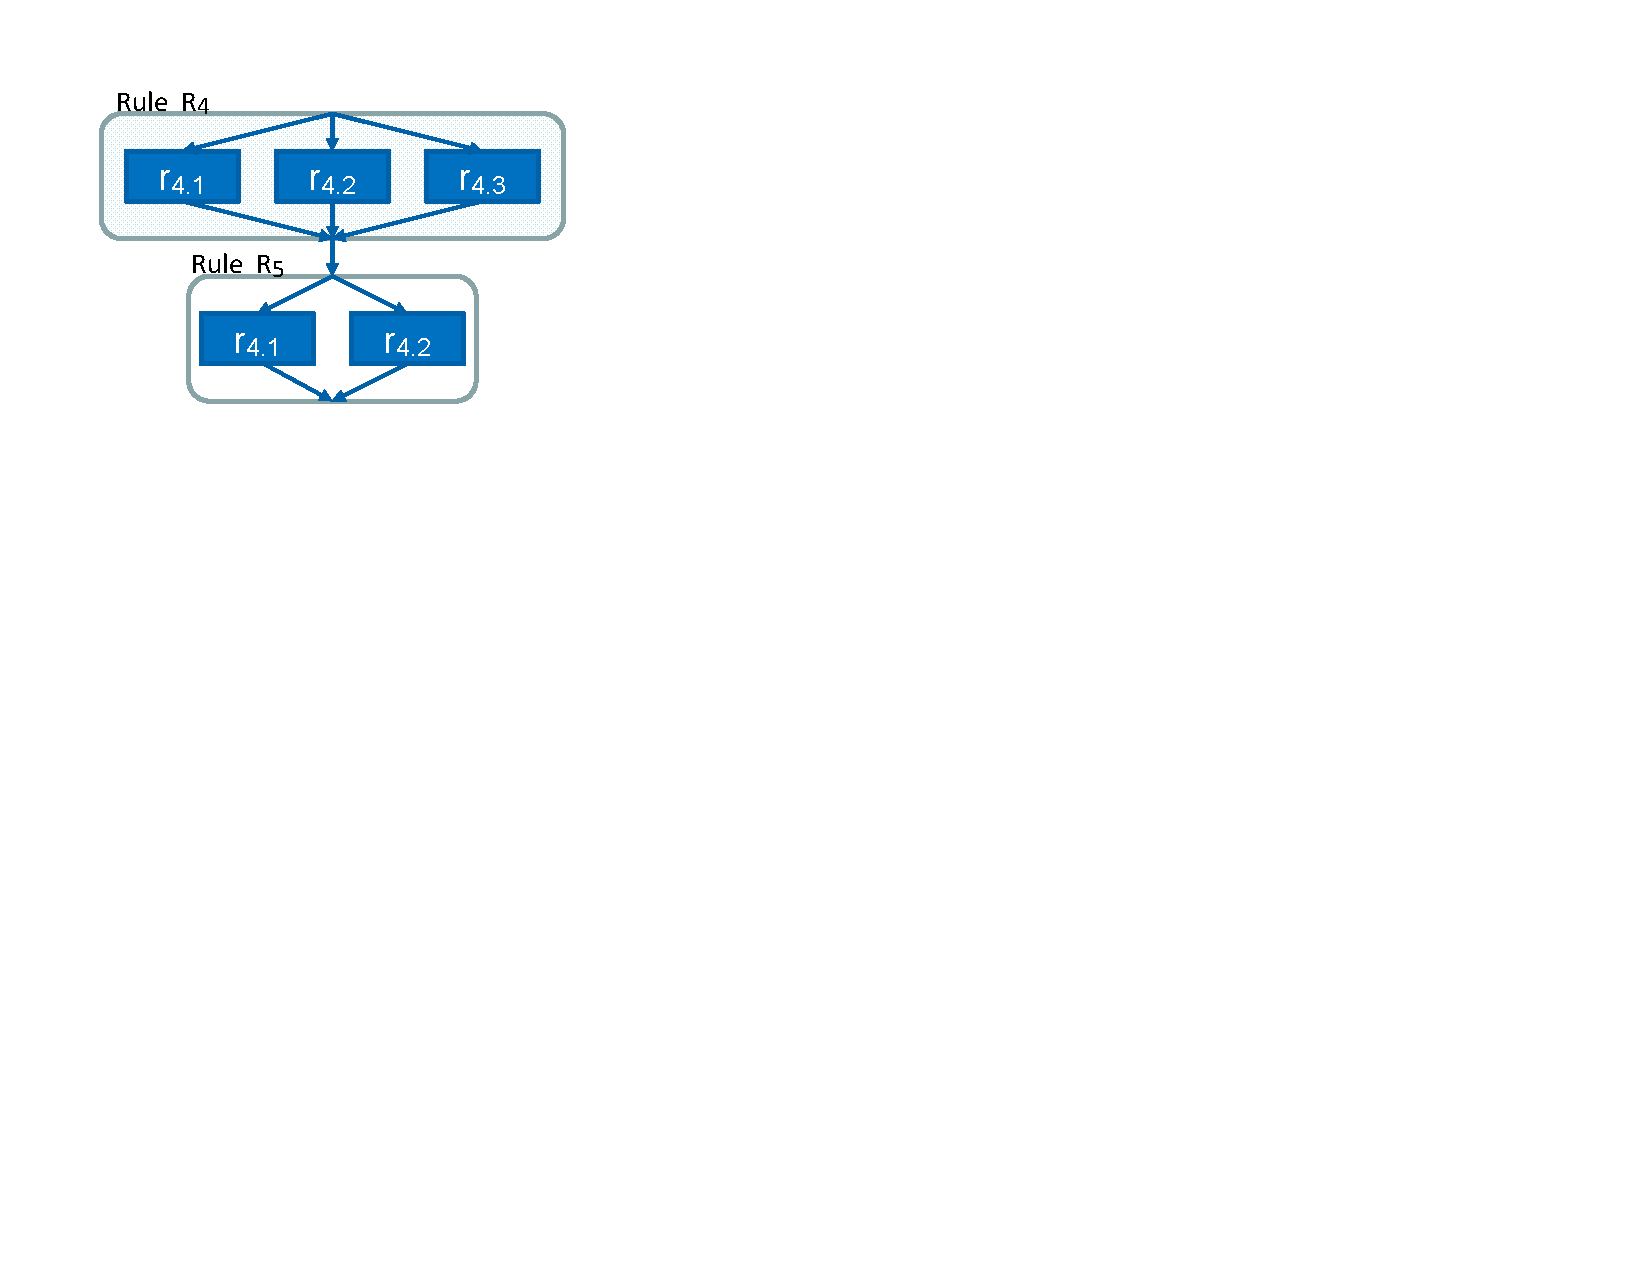
\includegraphics[trim=45 310 430 38,clip,width=3in]{figs/cfg-example.pdf}
\caption{Example operation flow model.}
\label{fig:cfg}
\end{figure}

%\begin{figure*}
%%  \centering
  %\begin{subfigure}[b]{0.4\textwidth}
    %\centering
    %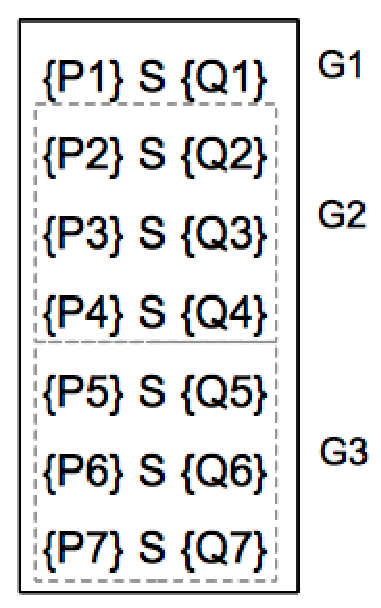
\includegraphics[width=.4\linewidth]{figs/cfg-example1}
    %\caption{An operation}
    %\label{fig:cfga}
  %\end{subfigure}%
  %\begin{subfigure}[b]{0.4\textwidth}
    %\centering
    %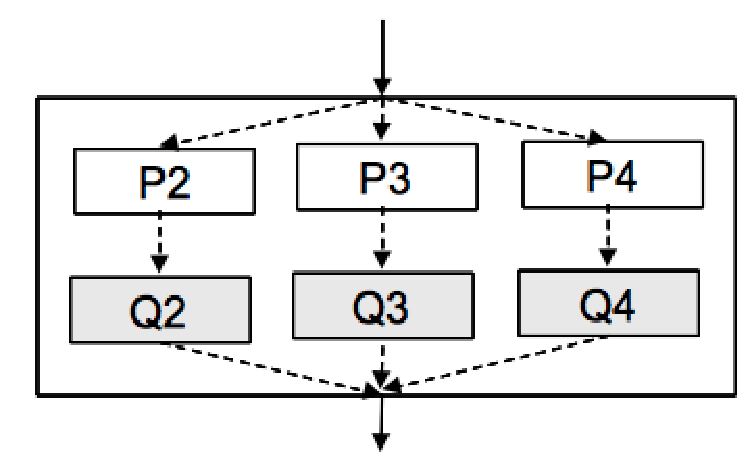
\includegraphics[width=.4\linewidth]{figs/cfg-example2}
    %\caption{The interopertational flow for group 2}
    %\label{fig:cfgb}
  %\end{subfigure}%
  %\begin{subfigure}[b]{0.2\textwidth}
    %\centering
    %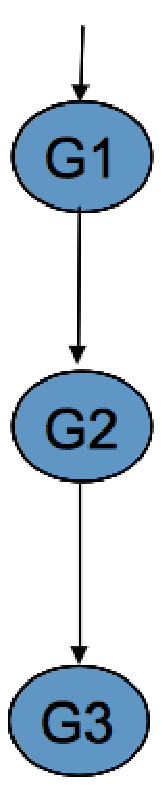
\includegraphics[width=.4\linewidth]{figs/cfg-example3}
    %\caption{The CFG component for the entire operation}
    %\label{fig:cfgc}
  %\end{subfigure}%
  %\caption{Control flow graph generation for a single operation}
  %\label{fig:cfg}
%\end{figure*}

%Some edges are specified directly by the designer of the model...next and triggers

\begin{algorithm}[t]
\SetAlgoVlined
\footnotesize
\KwIn{operation $op$, rule part $rp$}
\KwOut{operation sequence $seq$ or $null$}
\BlankLine

\nl Initialize a Queue $queue$ of sequences of operations\;
\nl Get all inputs of operation $op$\;
\nl Create all initialization sequences for all inputs of $op$\;
\nl Add all sequences to the Queue $queue$\;

\nl \While { queue not empty }
{
		\nl Remove the first sequence $fseq$ from the queue\;
		\nl seq = Invoke $CheckSequence$ ($fseq$) to check whether the sequence covers rule part $rp$\;
		\nl \If {seq is not null}
		{
				\Return seq\;
		}
		
		\nl Extract unsatisfied core of the sequence\;
		\nl Identify candidate operations $ops$ that help cover unsatisfied core\;
		
		\ForEach {Operation $candidate$ $\in$ $ops$}
		{
			\nl Insert $candidate$ to $fseq$\;
			\nl Add $fseq$ to Queue $queue$\;			
		}
}

\Return $null$\;
		
\caption{\label{alg:guidedsearch} Algorithm \lang{GuidedSearch} for
  identifying a sequence of operations that cover a given rule part.}
\end{algorithm}



\subsection{Technique}
\label{sec:technique}


\subsubsection{Binding.}
When sequencing two operations we need to substitute the entities
consumed by the successor operation by the entities created or
modified by the predecessor operation.

In our algorithm we move this problem to the underlying constraint
solver by creating constraints that bind the identifiers in the post
condition of the predecessor operation to the identifiers of same type
in the pre condition of the successor operation. As the solver has no
notion of objects, the binding must also ensure that object fields
referenced are appropriately bound.

Binding constraints are generated as follows: Assume that we want to
sequence the two operations $O_{pred}$ and $O_{succ}$ and that the
algorithm have chosen rules $r_1$ and $r_2$ from $O_{pred}$ and
$O_{succ}$ respectively for the sequencing. Now let $v$ be an
identifer of type $\tau$ occuring in either the creates or modfies
clause of $O_{pred}$ and let $w$ be an identifier of same type
occuring in the input clause of $O_{succ}$. If $\tau$ is an enum type,
the only binding needed is $w = v$. If $\tau$ is an object type, then
we must bind all subfields as well, yielding the following constraint:
$w = v \wedge w.f_1 = v.f_1 \wedge \ldots \wedge w.f_n = v.f_n$ where
$f_1, \ldots , f_n$ are fields declared on $\tau$. If any of the
fields are of object types themselves this process is applied
recursively on each such field to generate the final binding
constraint.

As an example of this process take the \emph{Compute Invoice Total}
operation shown in Figure~\ref{fig:invoice}... Include figure from
slide 12?
